 \documentclass[11pt]{book}

% \usepackage{amssymb}
% \documentclass[12pt,a4paper]{article}
% % \usepackage[subpreambles=true]{standalone}
% \usepackage[a4paper]{geometry}
% \usepackage[utf8]{inputenc}
% \usepackage[T1]{fontenc}
% \usepackage[light]{CormorantGaramond}
% \usepackage{import}
%
\linespread{1.1}

\usepackage{amsmath, amssymb, amsfonts, amsthm, mathtools}
\newcommand{\R}{\mathbb{R}}
\newcommand{\Z}{\mathbb{Z}}
\newcommand{\argmin}{\arg\!\min} % AlfC
\newcommand{\argmax}{\arg\!\max} % AlfC
\newcommand{\myeq}{\mathrel{\stackrel{\mbox{\normalfont\tiny{$\alpha \ll 1$}}}{\approx}}}
\DeclareMathOperator{\tr}{tr}
\newcommand{\irchi}[2]{\raisebox{\depth}{$#1\chi$}}
\newcommand{\rchi}{{\mathpalette\irchi\relax}}
\usepackage{algorithm}
\usepackage{algpseudocode}
\usepackage{float}

\usepackage{microtype} %improves the spacing between words and letters

\usepackage{lipsum}
\usepackage{threeparttable}
\usepackage{tabularx}
\usepackage{multirow}
\usepackage{booktabs}
\newcommand{\tabitem}{~~\llap{\textbullet}~~}
\usepackage{graphicx}
\graphicspath{ {./pics/} {./eps/}}
\usepackage{epsfig}
\usepackage{epstopdf}

%%%%%%%%%%%%%%%%%%%%%%%%%%%%%%%%%%%%%%%%%%%%%%%%%%
%% COLOR DEFINITIONS
%%%%%%%%%%%%%%%%%%%%%%%%%%%%%%%%%%%%%%%%%%%%%%%%%%
\usepackage[dvipsnames]{xcolor} % Enabling mixing colors and color's call by 'svgnames'
%%%%%%%%%%%%%%%%%%%%%%%%%%%%%%%%%%%%%%%%%%%%%%%%%%
\definecolor{MyColor1}{rgb}{0.2,0.4,0.6} %mix personal color
\definecolor{MyColor2}{HTML}{A30073}
\definecolor{MyColor3}{HTML}{A3008F}
\newcommand{\textb}{\color{Black} \usefont{OT1}{lmss}{m}{n}}
\newcommand{\blue}{\color{MyColor1} \usefont{OT1}{lmss}{m}{n}}
\newcommand{\blueb}{\color{MyColor1} \usefont{OT1}{lmss}{b}{n}}
\newcommand{\red}{\color{LightCoral} \usefont{OT1}{lmss}{m}{n}}
\newcommand{\green}{\color{Turquoise} \usefont{OT1}{lmss}{m}{n}}
%%%%%%%%%%%%%%%%%%%%%%%%%%%%%%%%%%%%%%%%%%%%%%%%%%

%%%%%%%%%%%%%%%%%%%%%%%%%%%%%%%%%%%%%%%%%%%%%%%%%%
%% FONTS AND COLORS
%%%%%%%%%%%%%%%%%%%%%%%%%%%%%%%%%%%%%%%%%%%%%%%%%%
%    SECTIONS
%%%%%%%%%%%%%%%%%%%%%%%%%%%%%%%%%%%%%%%%%%%%%%%%%%
\usepackage{titlesec}
\usepackage{sectsty}
%%%%%%%%%%%%%%%%%%%%%%%%
%set section/subsections HEADINGS font and color
\newcommand*{\myfont}{\fontfamily{cmr}\selectfont}
\chapterfont{\myfont \color{MyColor1}}
\sectionfont{\myfont \color{MyColor1}}
\subsectionfont{\myfont\color{MyColor1}}  % sets colour of sections

%set section enumerator to arabic number (see footnotes markings alternatives)
% \renewcommand\thechapter{\arabic{chapter}.} %define chapters numbering
% \renewcommand\thesection{\arabic{section}.} %define sections numbering
% \renewcommand\thesubsection{\thesection\arabic{subsection}} %subsec.num.

%%%%%%%%%%%%%%%%%%%%%%%%%%%%%%%%%%%%%%%%%%%%%%%%%%
%		CAPTIONS
%%%%%%%%%%%%%%%%%%%%%%%%%%%%%%%%%%%%%%%%%%%%%%%%%%
\usepackage{caption}
\usepackage{subcaption}
\usepackage{sidecap}
\sidecaptionvpos{figure}{c}
%%%%%%%%%%%%%%%%%%%%%%%%
\graphicspath{{./figures/}} %Setting the graphicspath
% \graphicspath{{./figures/G&D/}} %Setting the graphicspath
% \captionsetup[figure]{labelfont={color=Turquoise}}

%%%%%%%%%%%%%%%%%%%%%%%%%%%%%%%%%%%%%%%%%%%%%%%%%%
%		!!!EQUATION (ARRAY) --> USING ALIGN INSTEAD
%%%%%%%%%%%%%%%%%%%%%%%%%%%%%%%%%%%%%%%%%%%%%%%%%%
%using amsmath package to redefine eq. numeration (1.1, 1.2, ...)
%%%%%%%%%%%%%%%%%%%%%%%%
\renewcommand{\theequation}{\thesection\arabic{equation}}

%set box background to grey in align environment
\usepackage{etoolbox}% http://ctan.org/pkg/etoolbox
\makeatletter
\patchcmd{\@Aboxed}{\boxed{#1#2}}{\colorbox{black!15}{$#1#2$}}{}{}%
\patchcmd{\@boxed}{\boxed{#1#2}}{\colorbox{black!15}{$#1#2$}}{}{}%
\makeatother
%%%%%%%%%%%%%%%%%%%%%%%%%%%%%%%%%%%%%%%%%%%%%%%%%%

\makeatletter
\let\reftagform@=\tagform@
\def\tagform@#1{\maketag@@@{(\ignorespaces\textcolor{red}{#1}\unskip\@@italiccorr)}}
\renewcommand{\eqref}[1]{\textup{\reftagform@{\ref{#1}}}}
\makeatother
\usepackage{hyperref}
\hypersetup{colorlinks = true, linkcolor  = black}

%% LISTS CONFIGURATION %%
\usepackage{enumitem}
\setlist[enumerate,1]{start=1}
\renewcommand{\labelenumii}{\theenumii}
\renewcommand{\theenumii}{\theenumi.\arabic{enumii}.}
\newcommand{\cri}[1]{\textcolor{MyColor2}{\textbf{(Cri says: #1)}}}

%%%%%%%%%%%%%%%%%%%%%%%%%%%%%%%%%%%%%%%%%%%%%%%%%%
%% abbreviations:
%%%%%%%%%%%%%%%%%%%%%%%%%%%%%%%%%%%%%%%%%%%%%%%%%%
\usepackage[acronym]{glossaries}
\newacronym{pca}{PCA}{Principal Component Analysis}
\newacronym{mimo}{MIMO}{Multiple-input Multiple-output}
\newacronym{bs}{BS}{Base Station}
\newacronym{ut}{UT}{User Terminal}
\newacronym{csi}{CSI}{Channel State Information}
\newacronym{iot}{IoT}{Internet if Things}
\newacronym{m2m}{M2M}{Machine to Machine}
\newacronym{3gpp}{3GPP}{3rd Generation Partnership Program}
\newacronym{fdd}{FDD}{Frequency Division Duplex}
\newacronym{tdd}{TDD}{Time Division Duplex}
\newacronym{ce}{CE}{Channel Estimation}
\newacronym{ul}{UL}{Uplink}
\newacronym{sinr}{SINR}{Signal-to-Interference plus Noise Ratio}
\newacronym{sir}{SIR}{Signal-to-Interference Ratio}
\newacronym{evd}{EVD}{Eigenvalue Decomposition}
\newacronym{map}{MAP}{Maximum a-posteriori}
\newacronym{cdma}{CDMA}{Code Division Multiple Access}
\newacronym{snr}{SNR}{Signal to Noise Ratio}
\newacronym{svd}{SVD}{Singular Value Decomposition}
\newacronym{ber}{BER}{Bit Error Rate}
\newacronym{qpsk}{QPSK}{Quaternary Phase Shift Keying}
\newacronym{4g}{4G}{Fourth Generation}
\newacronym{srs}{SRS}{Sounding Reference Signal}
\newacronym{ofdm}{OFDM}{Orthogonal Frequency Division Multiplexing}
\newacronym{fr}{FR}{Fractional Reuse}
\newacronym{frcc}{FR-CC}{Cell-centric Fractional Reuse}
\newacronym{frna}{FR-NA}{Neighbour-aware Fractional Reuse}

\makeatletter
\newcommand{\chapterauthor}[1]{%
  {\parindent0pt\vspace*{-25pt}%
  \linespread{1.1} \scshape#1%
  \par\nobreak\vspace*{35pt}}
  \@afterheading%
}
\makeatother


\begin{document}
% \tableofcontents

\chapter{The Pilot Contamination problem}
\chapterauthor{Author Name (Cristina Gava)\\
Student ID 1153449}

\section{Overview}
Compared to existing cellular network infrastructures, nowadays there is an increasing need for technologies providing higher capacity. This comes from an always bigger demand for higher data rates in wireless mobile communication systems such as \gls{iot}, \gls{m2m} communication and other electronic services.

The current 4G cellular networks, \gls{3gpp} above all, were designed with the intention to support a peak spectral efficiency of $15$ bps/Hz, a bandwidth of $100$ MHz and an ultra-low latency. Nonetheless, the estimated future traffic far exceeds the resources of the current 4G and so the need for 5G cellular networks.

One of the novelties of the 5G protocol which is beeing designed and refined in the present communication scenario is the \gls{mimo} system, a technology that focuses on the idea of implementing multiple antennas terminals in one device - or \gls{bs} - in order to enhance the quality and reliabilty of communication. Without going into details, one of the options for this system is the multiuser \gls{mimo} system, where and array of antennas serves a group of autonomous terminals at the same time. These terminals may be single-antenna cheap devices and the multiplexing throughput gains are shared among the \gls{ut}s \cite{Marzetta2010} \cite{Elijah2016}.

In this type of system, the \gls{csi} has a crucial role, since forward-link data transmission needs that the base station know the forward channel, as well as the reverse-link data transmission require it to know the reverse channel. This is the reason why such things as pilot signals exist, but with them some problems might arise due to the contamination of such signals. What we mean to takle in this chapter is exactly to have a detailed look at those kind of problems, referred to as pilot contamination, and at a couple of main approaches to solve them.

\section{The pilot contamination problem}
In several works multi-user \gls{mimo} operations with a big excess of base station antennas are considered: in them the channel is estimated exploiting the feedback or channel reciprocity schemes through multiplexing over frequency - \gls{fdd} - or over time - \gls{tdd}. In \gls{tdd} a time-slot, over which the channel can be thought as constant, is divided between reverse-link pilots and forward-link data transmission. The pilots assume reciprocity to provide the \gls{bs} with an estimate of the forward channel, which in turn generates a linear pre-coder for data transmission \cite{Marzetta2010}. In the \gls{fdd} scenario, the division is made over the frequency and the system requires not only the estimation, but also feedbacks for both forward and reverse direction between the \gls{bs} and the \gls{ut}.

For this reason \gls{tdd} is considered a more suitable approach the \gls{fdd} when it comes to acquiring \gls{csi} in wireless systems \cite{Elijah2016} and following this line, we will focus on this system.

In \gls{tdd} the time pilots require is proportional to the number of terminals served, while the number of base station antennas does not influence it. At the same time, though, the number of terminals that can be served is limited by the coherence time. One of the principal findings in this sense is that the addition of \gls{bs} antennas always brings benefits to the SNR situation.

To simplify the observed scenario, several works focus on multi-user \gls{mimo} operations with an infinite number of base station antennas in a multicellular environment. In general, in a massive \gls{mimo} system, when the \gls{ut}s transmit their pilot sequences to the \gls{bs} in order to perform the channel estimation in the \gls{ul} training phase, every \gls{bs} not only learns the channel related to the intended \gls{ut}, but also fractions of the channels connected to other \gls{ut}s that happen to have pilots which are related to the ones used by the intended \gls{ut}.

% In this frame, orthogonal pilots would need length of at least $K \times L$ symbols (with $K = $ overall number of \gls{ut}s in a cell and $L = $ total number of cells in a system) due to frequency reuse factor of one, so non-orthogonal pilots across neighboring cells are used. At the same time, the use of $K \times L$ pilots is not feasible beacuse of short channel coherence times due to \gls{ut}s mobility \cite{Elijah2016}. Because of it, the problem of pilot contamination arises and it has been considered one of the main impirments in massive \gls{mimo} systems.

\subsection{\gls{ul} training}
The use of pilot in the \gls{tdd} scheme is related to the Uplink segment training. Considering the worst-case scenarion in this means assuming that all \gls{ut}s transmit synchronous pilot sequences of length $\tau$ symbols at the beginning of every coherence interval. Every cell then transmits a $\tau \times K$ orthogonal matrix $\textbf{S}_j = (\textbf{s}_{j1},\dots,\textbf{s}_{jk})$ which satisfies $\textbf{S}_j^T\textbf{S}_j = \tau \textbf{I}$. The received signal matrix at the $l_{th}$ \gls{bs} is then:
\begin{equation}
\textbf{Y}_l = \sqrt{p_u}\sum_{j=1}^{L}\textbf{D}_{l,j}^{1/2}\textbf{H}_{l,j}\textbf{S}_j^T + \textbf{N}_l
\label{eq:recSignal}
\end{equation}
with:
\begin{itemize}
  \item $\textbf{N}_l = $ the $M \times \tau$ additive noise matrix whose elements are are i.i.d. zero mean, circularly-symmetric complex gaussian $\mathcal{CN}(0,1)$ random variables;\\
  \item $p_u = $ the average transmit power at each user on the uplink and is a measure of pilot signal-to-noise ratio;\\
  \item
  \begin{equation}
    \textbf{D}_{l,j} =
    \begin{bmatrix}
      \beta_{l,1,j} &        &              \\
                    & \ddots &              \\
                    &        & \beta_{l,K,j}\\
    \end{bmatrix}
  \end{equation}
  with $\beta_{l,k,j}$ being the large scale fading coefficient;\\
  \item
  \begin{equation}
    \textbf{H}_{l,j} =
    \begin{bmatrix}
      h_{l,1,j,1} & \dots  & h_{l,k,j,1}\\
      \vdots      & \ddots & \vdots\\
      h_{l,1,j,M} & \dots & h_{l,k,j,M}\\
    \end{bmatrix}
  \end{equation}
  with $h_{l,k,j,m}$ being the small scale fading factor whose variables are $\mathcal{CN}(0,1)$.\\
\end{itemize}
\section{The main sources of contamination}
Pilot conatmination can be related to two main causes: non-orthogonal pilot schemes and hardware impairments.
While the first source is the most common and known one, the second source has been considered only recently and is still gaining consideration.

\subsection{Non orthogonal pilot schemes}
Normally, in a multi-cell system where the same frequency is shraed by L users, pilots are assumed mutually orthogonal and hence the intra-cell intereference is considered negligible. However, when frequency reuse comes into play, these signals are affected by this intereference, resulting in pilot contamination. In this case, the expression for the received signal is tha same as in \ref{eq:recSignal} \cite{Elijah2016}.

The conclusion of inter-cell interference was reached already by Marzetta in \cite{Marzetta2010}, where he precisely excluded the other possible sources of intra-cell interference and shadow fading. The author starts from the already considered propagation model where the single-antenna terminals are randomly distributed over the cell and separated by hundreds of wavelengths. Under these assumptions, the propagation vectors between the base station and the different terminals would be uncorrelated, since for a sufficiently high number of elements in a base station array the typical angular spacing between any two terminals would be greater than the angular Rayleigh resolution of the array, resulting in asymptotically orthogonal propagation vectors for different terminals. In fact, it can be shown that the inner product between two propagation vectors of any two terminals has a standard deviation of $\sqrt{M}$ (with $M$ being the number of antennas at the \gls{bs}) and it can be related to the critical assumtpion that, as the number of base station antennas grows, this inner product grows at a lower rate that the inner products of propagation vectors with themselves.

Under this assumption, the intra-cell intereference, the fast fading and the additive receiver noise effect disappear, laving the inter-cell interference as the only remaning hobstacle.

In this context the author analiyses the transmission scenario where he considers:
\begin{itemize}
  \item Hexagonal cells;
  \item OFDM modulation;
  \item Unlimited number of antennas per \gls{bs};
  \item Single antennas terminals;
  \item \gls{tdd}.
\end{itemize}
Here the maximum number of terminals for which the \gls{bs} can learn the channel is limited by the time it takes to acquire the \gls{csi} from the moving terminals, specifically: $K_{max} = \tau N_{smooth}$ with $\tau$ the number of OFDM symbols and $N_{smooth}$ the time over which the channel response is constant. The implication is that in general pilots from different cells are non-orthogonal, unless, for $K$ pilots in the $l_{th}$ cell, $K\cdot L \leq \tau N_{smooth}$ is true. The main conclusion of this apporach is that the frequency reuse among cells makes this relation false, and so justifies the inter-cell interference as the main source of pilot contamination \cite{Marzetta2010}.
\subsection{Hardware impairments}
Some works studied the impairments that some hardware components in radio frequency chain are prone to; these impairments can affect the accuracy of the \gls{ce} with related pilot contamination. These works approached this contamination source modeling some sort of non-ideal behavior of each component, but with more attention to the system overall response. In general, one main study \cite{Bjornson2014} shows how the hardware impairments from the \gls{bs} are negligible, while the main component of it comes from the \gls{ut}s, which limit the capacity in massive \gls{mimo} systems af M grows large. In this scenario, the \gls{ul} non-ideal system model that takes into consideration the distorsion noise for the received signal $\textbf{y} \in \mathbb{C}$ at the \gls{bs}, considering the deterministic pilot signal $d \in \mathbb{C}$, is represented by:
\begin{equation}
  \textbf{y} = \textbf{g}(d + {\eta}_t^{UT}) + \mathbf{\eta}_r^{BS} + \textbf{v}
\end{equation}
Where the stochastic processes $\eta_t^{UT} \in \mathbb{C}$ and $\mathbf{\eta}_r^{BS} \in \mathbb{C}^{M\times 1}$ describe the impairments of the transmitter and the receiver hardware at the \gls{ut} and the \gls{bs} respectively. While the ergodic process which is the additive noise $\textbf{v} = \textbf{v}_{noise} + \textbf{v}_{interf} \in \mathbb{C}^{M\times 1}$ consists of independent receiver noise $\textbf{v}_{noise} \sim \mathcal{CN}(\textbf{0},\sigma_{BS}^2\textbf{I})$ and potential interference from other simultaneous transmissions.

\subsection{Effects of pilot contamination}
The effects that can be counted can be analyzed first by the formulation of \gls{sir} expressions that can subsequently be translated into achievable rates; As much as \gls{sinr} can be considered, which has been demonstrated to saturate as M tends to infinity both in the uplink and in the downlink segment \cite{Elijah2016} \cite{Buzzi}. At the same time system performance degrades visibly because pilot contamination when the inter-cell interference factor $\beta$, composed by shadow fading and path loss, increases \cite{Elijah2016}.
\section{Schemes for pilot contamination mitigation}
There are several existing methods which intend to eliminate or mitigate the effects of pilot contamination, in particular for the case of \gls{tdd} systems. The two main categories these solutions have been divided in are, namely, the pilot-based estimation approach and the subspace estimation approach. Below we will give a brief explanation of what the former method consists of, while we will present one solution for the latter.

\subsection{The pilot-based approach}
In this approach,the main idea is that non-orthogonal pilots are used across the cells, while orthogonal ones within the cell. Through this assumption it was possible, for example, to transmit pilot signals from different cells by shifting the pilot location in frames so that users in separate cells transmit Without overlapping in time. Another point of view is using precoding methods requiring a limited collaboration among the \gls{bs}s \cite{Elijah2016}.
\subsection{The subspace-based approach}
The strength of this approach is that it requires a very limited number of pilot symbols for operation. In these, \gls{csi} is obtained through the application of \gls{evd} on the covariance matrix of the received samples. Moreover, since is not true a priori that the desired channels are always stronger than the interfering channels, \gls{map} criteria were added to it in some solutions.

The solution we briefly consider here was elaborated by M\"uller \textit{et al.} in \cite{Ralf} and consists of a nonlinear channel estimation based on a subspace projection. One of the most important statements of the paper is the confutation of the conclusion drawn by Marzetta \textit{et al.} in \cite{Marzetta2010}, where they stated that the array gain cannot be achieved for channel estimation, but only for data detection. Disproving this, \cite{Ralf} uses this gain for the nonlinear channel estimation algorithm, as well as shows how pilot contamination is a consequence of linear channel estimation and not a fundamental effect that cannot be removed.

\subsubsection{System model}
The owrk considers a wireless communication channel in the \gls{ul}, with the channel bandwith smaller than the coherence bandwidth and the channel being frequency-flat, block-fading and narrowband. Let the number of trasmit antennas be T and the number of receiving antennas R $>$ T. In this context, we can elaborate the \gls{cdma} system:
\begin{equation}
  \mathbf{Y} = \mathbf{HX} + \mathbf{Z},
\end{equation}
where:
\begin{itemize}
  \item $\mathbf{X} \in \mathbb{C}^{T\times C}$ the transmitted data;
  \item $\mathbf{Y} \in \mathbb{C}^{R\times C}$ the received signal;
  \item $\mathbf{Z} \in \mathbb{C}^{R\times C}$ the additive noise;
  \item $\mathbf{H} \in \mathbb{C}^{R\times T}$ the channel matrix, whose columns denote the spreading sequences;
\end{itemize}
and we can deploy the well-know fact that there is no need to know the spreading sequences to demodulate the \gls{cdma}, to come up with a so-called blind approach described below.
\subsubsection{The proposed method}
The proposed algorithm states that it might be a good idea not to estimate the channel matrix $\mathbf{H}$, but directly consider the subspace channel:
\begin{equation}
  \mathbf{\tilde{Y}} = \mathbf{\tilde{H}X} + \mathbf{\tilde{Z}}
\end{equation}
and estimate the much smaller subspace channel matrix $\mathbf{\tilde{H}} \in \mathbb{C}^{t\times T}$.

This because only the largest eigenvalues of $\mathbf{Y}\mathbf{Y}^T$ are necessary to our purpose. In fact, considering the case of $T = 1$ active transmit antenna and looking for the matched filter $m^T$ such that the \gls{snr} at its output is maximum, we are indeed looking for maximizing the total received power normalized to the power gain of the filter. Mathematically:
\begin{equation}
  \mathbf{m} = \argmax_{\mathbf{m}}\frac{\mathbf{m}^T\mathbf{Y}\mathbf{Y}^T\mathbf{m}}{\mathbf{m}^T\mathbf{m}}
\end{equation}
And in such case, the maximum value is exactly given by the maximum eigenvalue of $\mathbf{Y}\mathbf{Y}^T$, for a result from the algebra.

If we now extend this idea to the case of multiple transmit antennas, we can see that the subspace of eigenvalues we need is given by the projection of the received signal onto the signal space basis $\mathbf{S}^T \in \mathbb{C}^{T\times R}$ which stands out by the matrix of left singular vectors obtained by \gls{svd} of $\mathbf{Y}$. To express it in a more formal way we have:
\begin{equation}
  \mathbf{Y} = \mathbf{U} \mathbf{\Sigma} \mathbf{V}^T
\end{equation}
with unitary matrices $\mathbf{U} \in \mathbb{C}^{R\times R}$ and $\mathbf{V} \in \mathbb{C}^{C\times C}$, and the diagonal matrix $\mathbf{\Sigma} \in \mathbb{C}^{R\times C}$ \cri{verifica l'insieme di appartenenza degli elementi di questa matrice} with diagonal entries sorted in non-increasing order. Based on this the $\mathbf{U}$ matrix has the structure:
\begin{equation}
  \mathbf{U} = [\mathbf{S|\mathbf{N}}]
\end{equation}
with the null space basis being $\mathbf{N} \in \mathbb{C}^{R\times (R-T)}$.

The projection in question is thus expressed as:
\begin{equation}
  \mathbf{\tilde{Y}} = \mathbf{S}^T\mathbf{Y}
\end{equation}
In this scenario, a remark on the white noise can be done and precisely that if then we consider the case of massive \gls{mimo} scenario, where $R >> T$, then we see that the influence of it onto the signal subspace becomes negligible as $R \rightarrow \inf$. This because white noise is evenly distributed in all dimensions of the full space, which in turn is much bigger than the T-dimensional signal subspace.

What is left then is the co-channel interference from L neighboring cells, which typically is not white and jusitfies the relation for which the more colored the smaller the \textit{load} factor:
\begin{equation}
  \alpha = \frac{T}{R}
\end{equation}
Were we able to identify which singular values correspond to channel vectors from inside the cell, as opposed to the ones from neighboring cells, we could try to remove them by subspace projection. Moreover, we keep also in mind that any R-dimensional channel vector from any transmitter to the receive array in the interested cell is orthogonal to any other channel vector. Thus we can conclude that, in a cellular system with power-controlled handoff strategy, the norm of channel vectors from neighboring cells can never be bigger than the norm of interested-cell channel vectors; this means that we can identify the singular values belonging to transmitters internal to the cell by ordering them by magnitude \cite{Ralf}.
\subsubsection{Performance ananlysis}
In this section we will give an approximate estimation of the number of transmit antennas which is suitable for for the previous approach.

In the frame of classical massive \gls{mimo} settings, with L finite, R,T $\rightarrow \inf$ and $0 \neq \alpha \ll 1$, the impairment process $\mathbf{Z}$ is composed by a white noise component $\mathbf{W}$ (having iid elements with zero mean and variance W) and the interference from L neighboring cells:
\begin{equation}
  \mathbf{Z} = \mathbf{W} + \mathbf{H}_I\mathbf{X}_I
\end{equation}
In our helps comes also the definition of the normalized coherence time:
\begin{equation}
  \kappa = \frac{C}{R}
\end{equation}
In the large antenna limit $R \rightarrow \inf$, if we consider that the singular values of the normalized noise $\frac{\mathbf{W}}{\sqrt{CW}}/$ are bounded by the interval
\begin{equation}
  \frac{1}{\sqrt{\kappa}} - 1 < x < \frac{1}{\sqrt{\kappa}} + 1
\end{equation}
we can say that, at most, the power of white noise being present in $\mathbf{\tilde{Y}}$ is:
\begin{equation}
  Noise_w = \left(\Big(\frac{\mathbf{W}}{\sqrt{CW}}\Big)\sqrt{CW}\right)^2 = CW\left(1+\frac{1}{\sqrt{\kappa}}\right)^2
\end{equation}
for one singular value, while it is
\begin{equation}
  TNoise_w
\end{equation}
in the worst case, where the T largest singular values of the noise affect the signal of interest.

To then calculate the \gls{snr} in $\mathbf{\tilde{Y}}$ we can give an espression for the total power of the received signal as $TRCP$, since the data signal $\mathbf{X}$ is iid zero mean with variance (which account for its power) $P$. The \gls{snr} can be thus lower bounded by:
\begin{equation}
  SNR \geq \frac{P}{W}\frac{R}{\left(1+ \frac{1}{\sqrt{\kappa}}\right)^2}
\end{equation}


As mentioned at the beginning of this section, there is also the co-channel interference from neighboring cells, which is not white but at the same time higly concentrated in certain subspaces and can be suppressed making use of the phase transition of spectra of large random matrices. Specifically, in \cite{Ralf2012} the authors show how, in a multiuser \gls{mimo} scenario, the eigenvalue distribution of $\mathbf{H}$, when properly scaled or shifted, separates into two separate non-overlapping bulks with each bulk being shaped very similar to the cases of pure scattering and pure line-of-sight. This comes to our help when trying to separate the co-channel interference (the equivalent of the pure scattering) from the normalized signal of interest $\frac{\mathbf{HX}}{\sqrt{TR}}$ (the equivalent of pure line-of-sight).

For this we start observing that in the appendix A of \cite{Ralf}, the signal of interest is shown to converge to:
\begin{equation}
  \mathcal{P} = \left[\frac{\kappa P}{\alpha}-2P\sqrt{\frac{\kappa^2 + \kappa}{\alpha}};\frac{\kappa P}{\alpha} + 2P\sqrt{\frac{\kappa^2 + \kappa}{\alpha}}\right]
\end{equation}
as $R \rightarrow \inf$ and for $\alpha \ll 1$.

We then proceed supposing the entries of the matrix of interfering signals $\mathbf{X}_I$ be iid with zero mean and variance $P$, while the entries of the matrix of interfering channels $\mathbf{H}_I$ be iid with zero mean and variance $I/P$. In this way the ratio accounts for the relative attenuation between the intercell users and users external to the cell and thus the empirical distribution of the squared singular values of the normalized co-channel interference ($\frac{\mathbf{H}_I\mathbf{X}_I}{\sqrt{TR}}$) converges to a limit distribution as well. This distribution, for $\alpha \ll 1$ is supported in the interval
\begin{equation}
  \mathcal{I} =  \left[\frac{\kappa I}{\alpha}-2I\sqrt{L\frac{\kappa^2 + \kappa}{\alpha}};\frac{\kappa I}{\alpha} + 2I\sqrt{L\frac{\kappa^2 + \kappa}{\alpha}}\right]
\end{equation}
Therefore, having obtained two intervals (and so relative upper bounds) on the signal received and the co-channel interference, we can make use of the statement in \cite{Ralf2012} to affirm that if these two intervals do not overlap, i.e.
\begin{equation}
  \mathcal{P}\cap \mathcal{I} = 0
\end{equation}
or better
\begin{align}
  \frac{P}{I} &> \frac{1 + 2\sqrt{\alpha L \left( 1 + \frac{1}{\sqrt{\kappa}} \right)}}{1 - 2 \sqrt{\alpha \left( 1 + \frac{1}{\kappa} \right)}}\\
  &\myeq 1 + 2 \left( 1 + \sqrt{L} \right)\sqrt{\alpha \left( 1 + \frac{1}{\kappa} \right)}
  \label{eq:cochannel}
\end{align}
then, in the limit $\alpha \rightarrow 0$ the signal bulk can always be separated from the interference one as long as $\frac{P}{I} > 1$. Through this it can be stated that the two subspaces, the signal and the interference one, can be identified blindly and the interference can be nulled out \cite{Ralf}.
\subsubsection{Results}
The results of M\"uller \textit{et al.} in \cite{Ralf} are obtained through the application of Monte-Carlo simulation for the undecoded \gls{ber} under the hypothesis of \gls{qpsk} and flat Rayleigh fading. These results have then been compared with the ones obtained by Marzetta in \cite{Marzetta2010}. In \autoref{fig:SNR} the case of high SNR is considered and shows how the \gls{ber} drops drastically if the reciprocal of the rate given in \ref{eq:cochannel} is below the threshold provided by the random matrix method, confirming the possibility to overcome the pilot contamination problem.

\autoref{fig:BER} represents the more relevant case, where the algorithm presented above achieves significant performance gains compared to the linear channel estimation. In the picture it is also underlined the maximum $I/P$ ratio over which the the singular values do not separate in the simulations.

\begin{SCfigure}
  \centering
  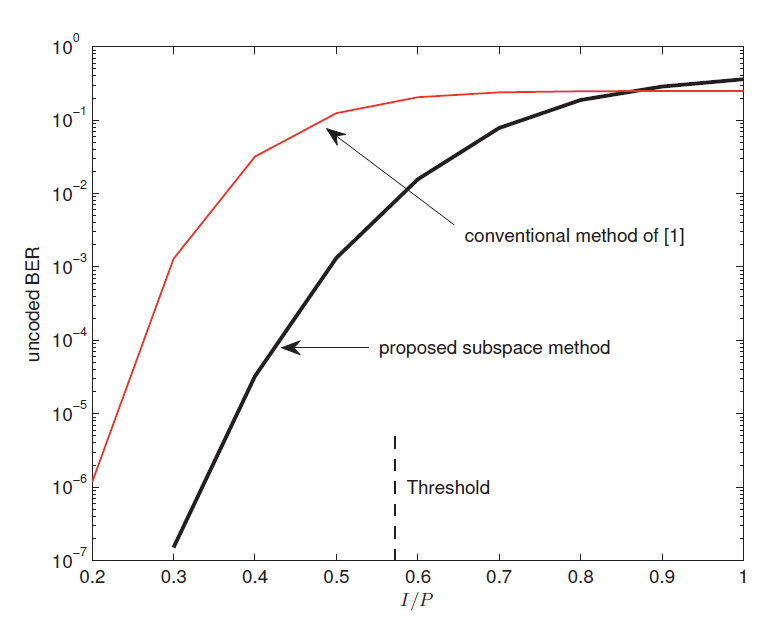
\includegraphics[width = 0.7\textwidth]{SNRvsMarzetta.png}
  \caption{\footnotesize{BER for 1 pilot symbol per transmit antenna and cell, $R = 400$
  receive antennas, $T = 4$ transmit antennas, $L = 2$ neighboring cells, coherence time  of $C = 1000$ symbols, and signal-to-noise ratio $P/W = 100$.}}
  \label{fig:SNR}
\end{SCfigure}
\begin{SCfigure}
  \centering
  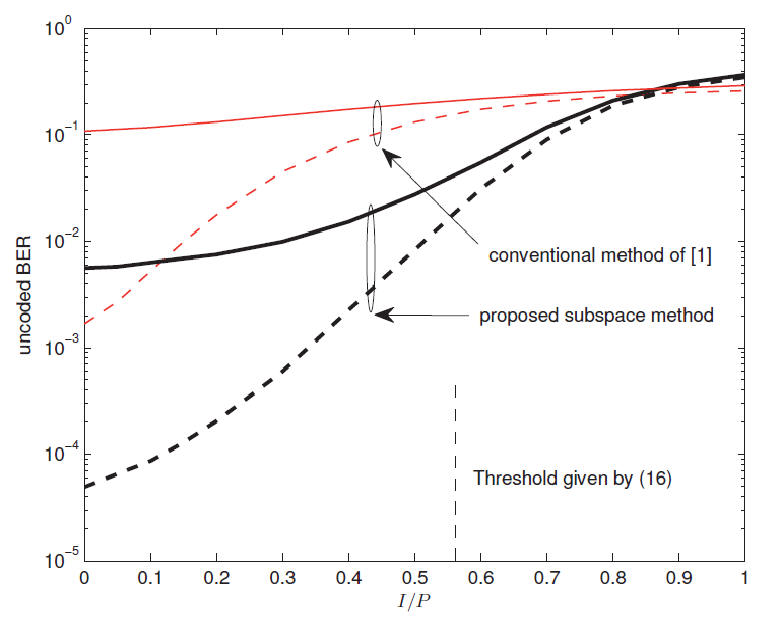
\includegraphics[width = 0.7\textwidth]{BERvsMarzetta.png}
  \label{fig:BER}
  \caption{\footnotesize{BER for $R = 200$ receive antennas, $T = 2$ transmit antennas, $L = 2$ neighboring cells, coherence time of $C = 400$ symbols, and signal-to-noise ratio $P/W = 0.1$. The solid and dashed lines refer to 1 and 10 pilot symbols per transmit antenna and cell, respectively.}}
\end{SCfigure}

\section{Pilot contamination and mmWaves}
As the last thing we tackle, a quite recent work from Naqvi \textit{et al.} focuses on the problem of pilot contamination in the mmWaves scenario \cite{Ahsan2016}.
\subsection{The scenario}
The authors use an hexagonal geometry with random deployment of users, studying a conventional frequency reuse and deriving the network throughput. The geometry and reuse model are well represented in \autoref{fig:geometry}, where each color represents a set of orthogonal pilots, which are in turn mutually orthogonal from color to color. The total number of cell in our case is $L$, the reuse factor of each cell is given by the parameter $Q = \{1,3,4,7,\dots\}$ and each cell contains an $M$-antenna \gls{bs} that serves K randomly deployed single antenna mobiles.
\begin{figure}
\centering
  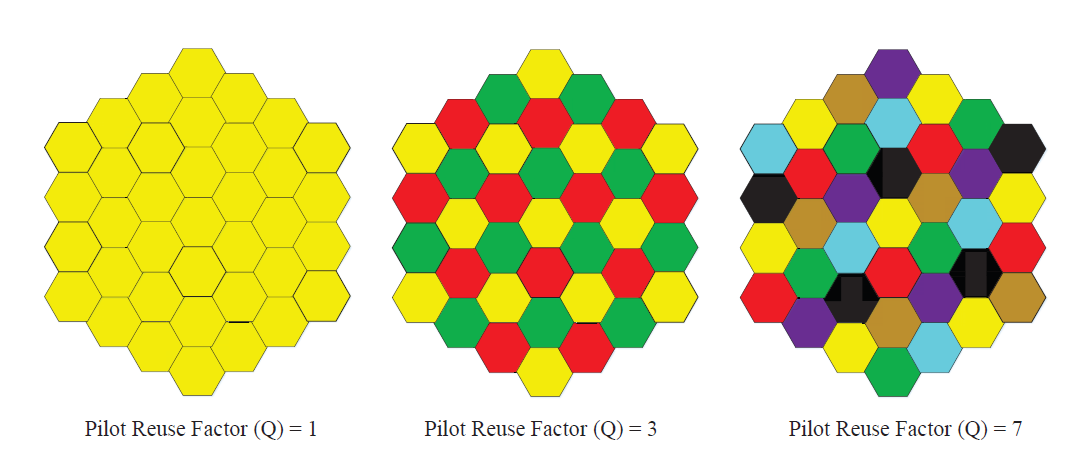
\includegraphics[width = .7\textwidth]{geometry.png}
  \caption{Pilot reuse under consideration}
  \label{fig:geometry}
\end{figure}
\subsection{Multicell \gls{ul} communication}
All the users in this scenario communicate with their respective \gls{bs} in two stages: the \gls{ul} training with pilot reuse and the actual transmission of data stage.

In the first stage orthogonal pilots are assigned to the users in each cell, and deploy the reuse factor $Q$. Specifically, assume a pre-designed pilot sequence matrix in the form:
\begin{equation}
  \mathbf{\Psi} = [\psi_0,\psi_1,\dots,\psi_{Q-1}] \quad \in \mathbb{C}^{QK\times QK}
\end{equation}
with $\mathbf{\Psi}$ being divided among the cells and the $i^{th}$ element of it is assigned to the $i^{th}$ serving cell, so that the pilot sequence is further reused by cell $lQ$, with $1 \leq |l| \leq \lfloor\frac{l}{Q}\rfloor$.

If we now take the case of cell $0$, for brevity, in a single-time frequency block, then the signals received at \gls{bs} $0$ are in the form:
\begin{equation}
  \mathbf{P}_0 = \sqrt{\phi_{\tau} QK}\sum_{j=0}^{L-1}\mathbf{H}_{0,j}\mathbf{\Psi}_{(j)}^* + \mathbf{W}_0 \quad \in \mathbb{C}^{M\times K}
\end{equation}
with, again, $H_{0,j}$ being the channel matrix between the mobiles of cell $j$ and \gls{bs} $0$, $\mathbf{W}_0$ being the iid $\mathcal{CN}(0,1)$ and $\phi_{\tau}$ being the average transmission power per mobile. We specify also that the factor $\sqrt{QK}$ guarantees that the average power is indeed $\phi_{\tau}$.

Next, the received signal is projected onto $\Psi_{0,k}$ in order to estimate the elements of $H_{0,j}$ at the \gls{bs} $0$.

The subsequent actual transmission of data works in a similar way and the expressions obtained in \cite{Ahsan2016} well distinguish the intra-dell and the inter-cell interfernce.

Finally, the reader can look at section $C$ in \cite{Ahsan2016} for the mathematical derivation of the achievable cell throughput.

\subsection{Results}
\begin{figure}
\begin{minipage}{.47\textwidth}
\centering
  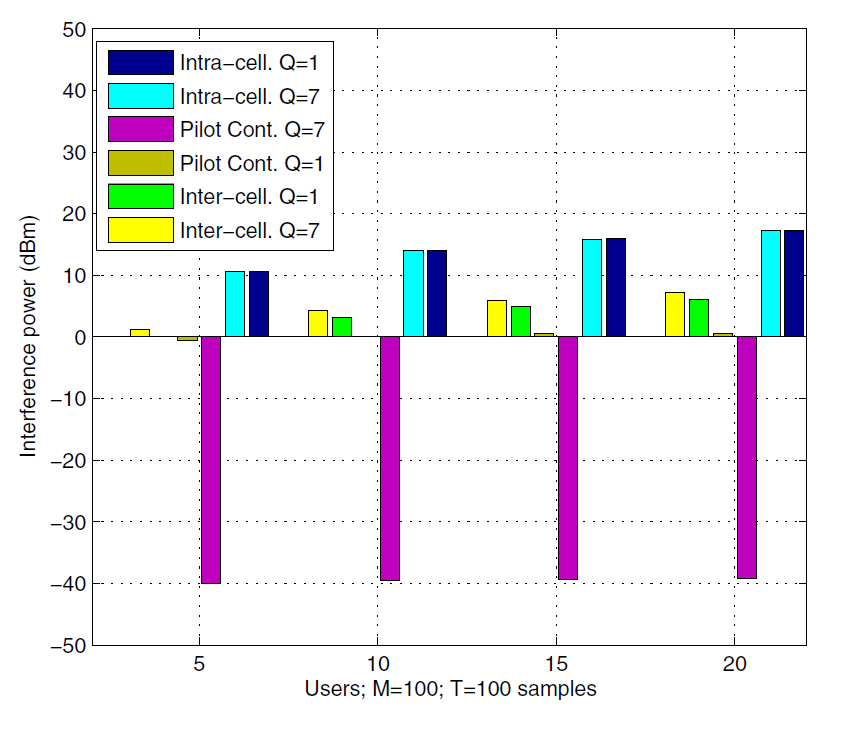
\includegraphics[width = \textwidth]{uhf.png}
  \caption{\footnotesize{Interference components in UHF systems using $Q = 1$ and $7$}}
  \label{fig:uhf}
\end{minipage}
\vspace{20mm}
\begin{minipage}{.47\textwidth}
\centering
  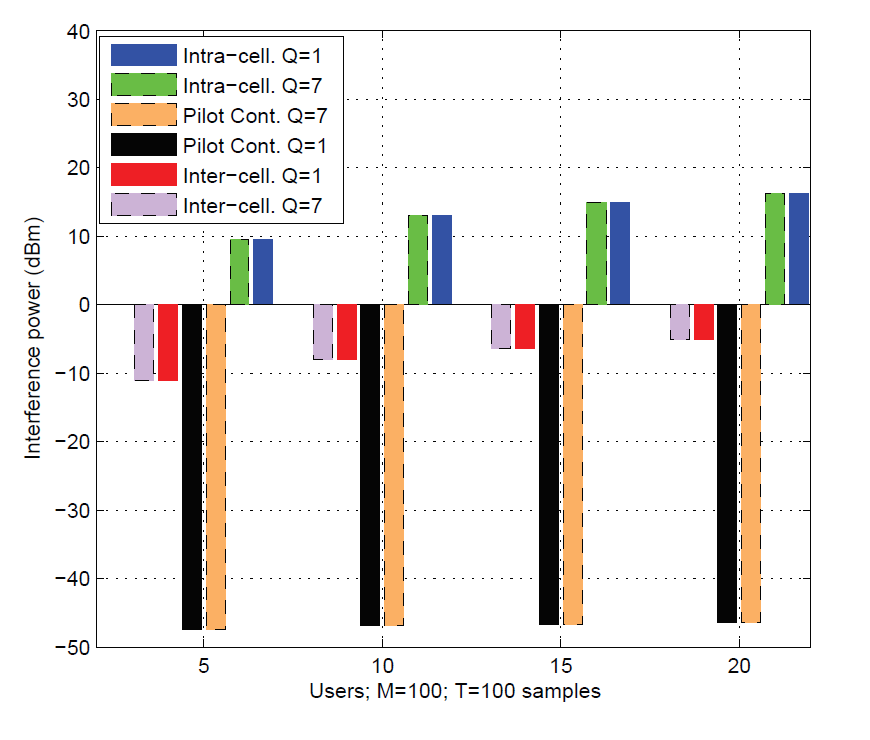
\includegraphics[width = \textwidth]{mm.png}
  \caption{\footnotesize{Interference components in mmWave systems using $Q = 1$ and $7$}}
  \label{fig:mm}
\end{minipage}
\end{figure}

We highlight here some of the most important results that come up from the work in \cite{Ahsan2016}. In the first chart in \autoref{fig:uhf} we can see the interference power for the UHF link for 5, 10, 15 and 20 users per cell, and $M = 100$ antennas. We put the focus on some main aspects:
\begin{itemize}
  \item the inter-cellular and the intra-cellular interferences
  increase steadily with an increase in the number of users for
  either value of $Q$. In this, since the user location is random, both the interferences have the same impact on the throughput: for closer points to the \gls{bs} the intra-cell interference dominates, while it is the contrary for long distances;
  \item the pilot contamination has separate fixed values for the
  two reuse factors that are independent of the total number of users. In this particular case, because of the hexagonal geometry the number of interferers causing pilot contamination will always be six for any reuse factor;
  \item what is most interesting, though, is the counterintuitive aknowledgment of the pilot reuse potency, as pilot contamination falls from approximately 0dBm for $Q=1$,to -40dBm for $Q=7$. This because a greater value of the pilot reuse factor, means a greater the distance of the interferer from the BS, and so, a greater path loss experienced by
  the interfering signal and, which means lesser pilot contamination.
\end{itemize}
In the second chart interference power for mmWave frequencies is examined. Here we see that:
\begin{itemize}
  \item there is a correspondence in inter-cellular
and intra-cellular interferences to the behavior seen in UHF systems;
  \item however, in this case the inter-cellular interference for both pilot reuse factors is much smaller than the one in the previous graph. These results allude to the advantage afforded by the mmWave link’s increased path loss, which drowns out the interference from the neighboring cells to the extent that a higher pilot
  reuse factor has no further impact on pilot contamination.
\end{itemize}

Summarizing what seen here so far, it can be stated that the mmWave link outperforms the UHF link to the point that at such high bandwidht mmWave links need not incorporate pilot reuse into the network, since the network gives virtually similar results for all the values of $K$ used, both for $Q = 1$ and $Q=3$.

\section{The pilot mitigation problem in the 5G 3GPP standard}
The concepts seen so far are applied to the commercial standards of the latest wireless communication systems, starting from the \gls{4g} precursor, where \gls{csi} is acquired through pilots in a scheme called \gls{srs} and which is still considered the main candidate to carry \gls{ul} massive \gls{mimo} pilots in \gls{tdd} systems.

However, as we previously mentioned, \gls{srs} reuse is the main cause of pilot contamination, therefore the approaches mentioned above are some of the possible solutions for it. In particular, the most recent adopted solutions try to optimize the pilot reuse schemes while keeping the training overhead under control. In \cite{Giordano}, Giordano \textit{et al.} focus on these schemes, evaluating their performance and highlighting the best one. In particular, they focus on \gls{ul} \gls{srs}s that span the entire bandwidth to allow a wideband channel sounding and consider a $2\times$ time repetition factor as well as 8 possible cyclic shifts of the \gls{ul} \gls{srs}, such that a maximum of 16 \gls{ul} \gls{srs} can be multiplexed in one \gls{ofdm} symbol. 5G standardisation is currently discussing whether amendments to this framework are needed to effectively support massive MIMO applications.

\subsection{The \gls{srs} coordination - fixed reuse}
The already well know pilot reuse schemes are named \textit{Reuse 1} and \textit{Reuse 3} and depending on them we can obtain two different upper bounds in the expression:
\begin{equation}
  N_{K,b} \leq \left\lfloor \frac{N_{I,\tau}}{3\beta_{PR}+\beta_{SH}} \right\rfloor
\end{equation}
representing the number $N_{K,b}$ of scheduled \gls{ut}s at the \gls{bs} $b$, considering a maximum of $N_{P,\tau}$ orthogonal \gls{srs}s and $\tau$ \gls{ofdm} symbols. Here, the parameter accounting for the reuse scheme type is $\beta_{PR} \in [0,1]$ and denotes the fraction of protected \gls{srs} sequences, which in turn are orthogonal among \gls{ut}s served by different \gls{bs}s. With this, $\beta_{SH} = 1 - \beta_{PR}$ is the remaining fraction of sequences that can be reused across the sectors of the same deployment site.

In particular, in the \textit{Reuse 1} ($\beta_{PR} = 0$) scheme, all \gls{ut}s scheduled by all \gls{bs}s share the entire set of \gls{srs}s, but since orthogonality is only guaranteed among \gls{ut}s associated with the same \gls{bs}, pilots among \gls{ut}s connected to different \gls{bs}s are not orthogonal. The consequences of it are that the largest number of \gls{ut}s are multiplexed, but there is a more severe
pilot contamination.

With \textit{Reuse 3}, ($\beta_{PR} = 1$), three co-located \gls{bs} sectors within the same cell site use three different and orthogonal sets of \gls{srs}s, so that pilot orthogonality is preserved across the entire cell site. Thus this scheme leads to lower pilot contamination with respect to \textit{Reuse 1} scheme, even though this effect comes at the expense of training only one third of the UEs given a fixed $\tau$, or alternatively, using three times as many \gls{ofdm} symbols $\tau$ when considering a fixed number of scheduled \gls{ut}s per \gls{bs}.

\subsection{The \gls{srs} coordination - fractional reuse}
The tradeoff between the previous schemes is represented by the so-called \textit{\gls{fr}}, in which \textit{Reuse 3} is applied for a specific fraction of \gls{ut}s $\beta_{PR}$ and the \textit{Reuse 1} for the remaining fraction$\beta_{SH}$, with the result of being able to multiplex a larger number of
sequences than \textit{Reuse 3} while providing less pilot contamination than \textit{Reuse 1}.

The two main \gls{fr} reuse schemes are:
\begin{itemize}
  \item The \textbf{\gls{frcc}}
  \item And the \textbf{\gls{frna}}
\end{itemize}

\bibliographystyle{ieeetr}
\bibliography{myBib}

\end{document}
